\chapter{Introduction and Literature Review}

% =============================================================
% PART A — INTRODUCTION
% =============================================================

%% MARQUEZ START
\section{Background of the Study}
The public transportation system has long been a commodity to people; it operates on different terrains, has different forms, and has predetermined routes depending on their geographical location and the needs of commuters \cite{Tironi2018}. With an increase in urbanization over time, the demand for transportation has also increased. Despite the predicted decline in urbanization rates in Southeast Asia, the Philippines is experiencing the opposite \cite{UN_WUP2018}. Due to the increased urbanization and the continuous increase in population (especially in urban areas), people start looking for different alternatives in transportation \cite{Cervero2000}. With the increasing number of motor vehicles on the road, the traffic congestion worsens, which leads to commuters finding other means to quickly reach their destination. In Metro Manila, severe traffic congestion, stemming from insufficient road infrastructure and poor traffic mitigation policies, has resulted in a highly inefficient public transport system \cite{Spatio2026}. As a response, the Philippine government launched the EDSA Bus Carousel in 2020. It is the only busway system in Metro Manila implemented by the government to have a designated lane, and separated from other cars by concrete barriers \cite{Chua2026}. Throughout the years of implementation, a large number of commuters have utilized the system with an average of 183,000 daily passengers, climbing up to 320,000 during peak periods, with a ridership of nearly 67 million in 2025, up from 63.02 million in 2024 (Figure~\ref{fig:bg-ridership}) \cite{DOTr2025Ridership}. With that amount of ridership, the EDSA Bus Carousel can be safely assumed to be one of the backbones of Metro Manila commuting.

\begin{figure}[htbp]
    \centering
    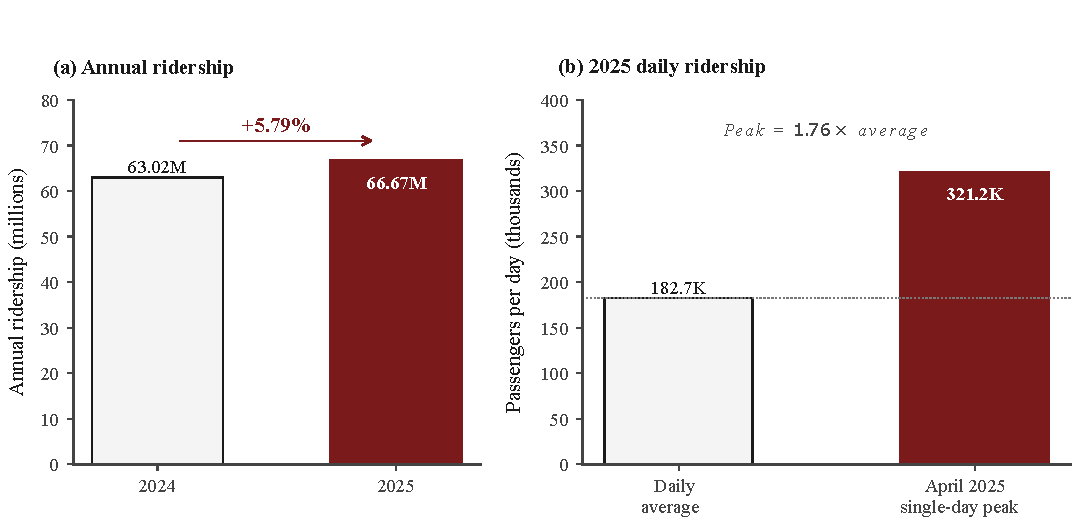
\includegraphics[width=0.95\textwidth]{Figures/bg_fig1_ridership.pdf}
    \caption[EDSA Carousel ridership]{EDSA Carousel ridership. (a) Annual ridership
    grew 5.79\% from 63.02M in 2024 to 66.67M in 2025. (b) Daily ridership in 2025
    averaged 182{,}655 passengers, with a single-day peak of 321{,}186 in April 2025
    --- approximately 1.76$\times$ the daily mean \cite{DOTr2025Ridership}.}
    \label{fig:bg-ridership}
\end{figure}
%%

Figure~\ref{fig:bg-corridor-map} shows the EDSA Carousel Southbound route from Monumento to PITX, the corridor this study is grounded in, together with the other public transport modes (jeepney, MRT, LRT, tricycle, UV/FX) that intersect it at each major stop.

\begin{figure}[htbp]
    \centering
    \includegraphics[width=0.75\textwidth]{Figures/bg_fig3_edsa_corridor_map.pdf}
    \caption[EDSA Carousel corridor map]{EDSA Carousel Southbound route
    (Monumento to PITX) with intersecting public transport modes at each
    stop. Authors' illustration, adapted from the group's defense
    presentation.}
    \label{fig:bg-corridor-map}
\end{figure}

Despite the gradual increase in demand, the EDSA Bus Carousel still faces a lot of significant operational issues that affect the quality of bus routing. Firstly, the LTFRB relied on a tedious manual monitoring process by deploying personnel at each stop, creating decisions through empirical observation. \cite{EDSApolicy2023}. In relation to that, it is also clear that bus bunching has not been resolved; most of the time, their designated dispatch schedule is not followed \cite{Ollero2024EDSA}. There is an acknowledged lack of a structured monitoring framework for operations (e.g., dispatching, dwell time, bus bunching), in which adjustments are often done only after recurring issues surface \cite{Tiglao2025}. Moreover, mechanical failures or bus breakdowns are also prominent in Metro Manila, which contributes to a stressful environment, highlighting that poor vehicle condition and the constant threat of mid-route breakdowns are significant chronic stressors for Filipino bus drivers \cite{Chua2026}. Furthermore, environmental stochasticity severely destabilizes operations: empirical studies on Philippine expressways show that increasing rainfall intensity significantly reduces average traffic speed and free-flow capacity \cite{TSSP_Rain2018}. This rainfall-impact evidence is drawn from a 2018 study of the North Luzon Expressway rather than the EDSA Busway, and is used here only as contextual motivation that weather materially affects Philippine road-traffic operations; the weather-disturbance generator in this study (Section~3.2.6) does not adopt this study's specific speed-reduction percentages, and EDSA-specific travel-time behavior is independently calibrated through the GEH/RMSE procedure described in Section~3.2.3.

\begin{figure}[htbp]
    \centering
    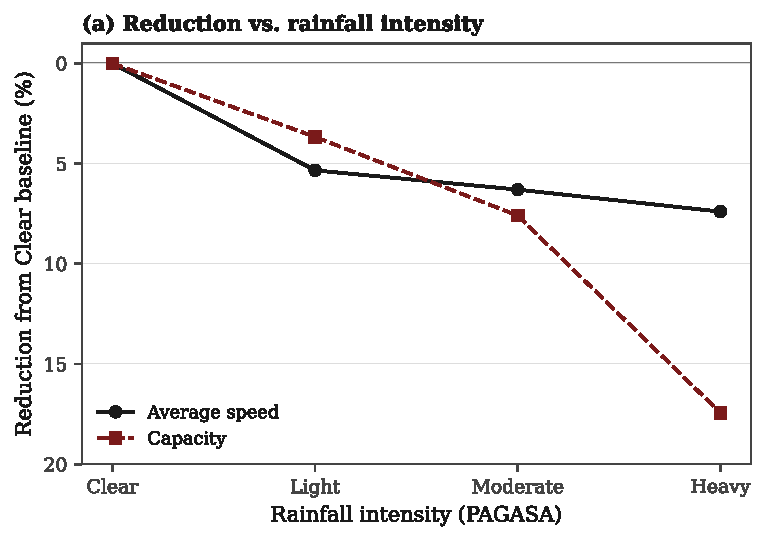
\includegraphics[width=0.7\textwidth]{Figures/bg_fig2_rainfall_traffic.pdf}
    \caption[Rainfall impact on traffic flow]{Reduction in average speed and
    free-flow capacity relative to the clear-weather baseline across PAGASA
    rainfall categories. Capacity loss grows sharply at heavy intensities
    ($-17.4\%$), whereas mean speed degrades more moderately ($-7.4\%$), adapted from \cite{TSSP_Rain2018}.}
    \label{fig:bg-rainfall}
\end{figure}

As Figure~\ref{fig:bg-rainfall} shows, the reduction in
average speeds are about 5.34\% under light rain conditions, 6.3\% under moderate rain
conditions, and 7.4\% under heavy rain conditions. The average volume decreased by 2.92\%,
10.62\%, and 12.39\% while the capacities reduced by 3.67\%, 7.6\%, and 17.44\% under light,
medium, and heavy rain conditions, respectively \cite{TSSP_Rain2018}. Severe weather events often initiate localized flooding at key segments like Muñoz and Monumento Stations or cause severe degradation, forcing operational halts and emergency speed restrictions that further affect the busway’s performance  \cite{PhilstarTyphoon2024, PIA_Emergency2023, BusRepair2023}. Given these operational hurdles, the bus dispatching process of the EDSA Carousel can be modeled as a Vehicle Scheduling Problem (VSP).

Traditionally, the VSP has been addressed through static scheduling, which utilizes fixed timetables and headways derived from historical averages \cite{Ceder2007}. However, these rigid, rule-based methods often fail in stochastic environments as they cannot adapt to real-time disruptions, necessitating a shift toward more dynamic, autonomous scheduling frameworks that can respond to the unpredictability of the corridor \cite{Ollero2024EDSA}. This motivated a transition toward data-driven methodologies. Initial studies utilized traditional machine learning (ML) for demand forecasting and traffic prediction \cite{Wang2017}, but these models are primarily limited to predictive tasks and lack the active control mechanisms required for real-time decision-making in a closed-loop system. The subsequent wave introduced Single-Agent Reinforcement Learning (SARL), which enabled autonomous control, yet these frameworks frequently suffer from the `curse of dimensionality' as the joint state and action spaces grow exponentially with the number of vehicles, leading to centralized bottlenecks that hinder scalability in large transit networks \cite{Chen2024Survey}. To overcome these limitations, Multi-Agent Reinforcement Learning (MARL) has emerged as the state-of-the-art approach, offering a decentralized execution framework that enables scalable, collaborative control among multiple buses to mitigate complex issues like bus bunching \cite{Wang2020Holding}.

Although recent studies have demonstrated the potential of MARL-based dynamic scheduling to improve transit adaptability and overall reliability, a critical research gap remains. Existing MARL bus scheduling models are primarily evaluated in controlled simulation settings and are typically tested against isolated disruptions. No prior work has evaluated these models under the combined, simultaneous severe disruptions such as heavy rain, mechanical breakdowns, traffic variations, and sudden passenger surges that portray real-world corridors like EDSA. Therefore, this study aims to evaluate a MARL-based dynamic bus scheduling model under these non-ideal, stochastic traffic conditions to mitigate bus bunching, minimize passenger waiting times, and improve overall dispatch efficiency on the EDSA Carousel.

%%MARQUEZ END
\clearpage
\section{Review of Related Work}
This section surveys prior work on data-driven bus and traffic scheduling using a funnel structure. It starts from the broad transition from static scheduling toward adaptive and learning-based control, narrows to single-agent reinforcement learning and its known scalability limitations in large transit systems, narrows further to Multi-Agent Reinforcement Learning (MARL) and the assumptions commonly used in existing MARL bus-scheduling studies, and finally identifies the robustness gap addressed in this study.

\subsection{From Static Rules to Machine Learning}
\textbf{Static scheduling} refers to the offline determination of bus departure times, headways, fleet allocations, and stop assignments based on historical demand and travel-time averages, fixed in advance of operations and not adjusted in real time in response to observed disturbances \cite{Ceder2007}. Once deployed, such schedules cannot react to live disturbances such as demand surges, congestion, weather-induced delays, or vehicle breakdowns. The poor performance of fixed timetables under such conditions is well documented: even-headway and schedule-based control degrade rapidly once travel-time and demand variability exceed the narrow band assumed at design time, allowing small headway perturbations to amplify into bunching \cite{Daganzo2009}. Static schedules therefore remain mathematically inadequate for stochastic traffic environments, where the governing quantities are random variables rather than deterministic constants. Under the specific non-ideal conditions this study targets, the failure modes differ by control strategy. A fixed timetable has no feedback mechanism at all, so once bunching begins nothing in the schedule corrects it. A local reactive rule that holds a bus based only on the gap to the bus ahead can partially correct bunching under ordinary congestion, but has no way to respond to a breakdown, since it observes only the forward gap and not the enlarged gap a failed bus leaves behind it. A more globally aware reactive rule that accounts for both the forward and backward gap improves on this, but still follows a fixed, pre-specified rule rather than a learned response, so it cannot adapt its behavior to the heavier-tailed delays that severe weather introduces. These limitations motivated the transition toward more adaptive and data-driven scheduling methodologies.

Machine Learning (ML) techniques subsequently emerged as important tools for improving operational responsiveness in transportation systems through demand estimation, traffic forecasting, predictive dispatching, and adaptive holding strategies \cite{huang2019,patil2025}. Unlike static scheduling approaches, ML-assisted frameworks incorporate continuously updated operational information to improve short-term decision support under uncertain traffic conditions \cite{huang2019}. Recent applications to transit operations have demonstrated measurable operational gains. Barrera Hernandez et al. applied passenger-demand forecasting to support a heuristic dispatcher for bus operations in Bogotá, reporting reductions in passenger waiting time and operational cost relative to fixed timetables \cite{Barrera2025Optimization}. Similarly, Usman et al. utilized ML-based density estimation to improve real-time responsiveness in public transit systems \cite{Usman2025ML}. These studies demonstrate the growing role of ML-assisted methodologies in adaptive transit scheduling and operational planning.

Despite these advances, many ML-assisted transit-control frameworks still rely heavily on manually engineered intervention logic and externally designed dispatch heuristics \cite{alexandre2023}. In several predictive-control and heuristic-dispatch systems, forecasting components improve operational visibility, but the resulting operational responses are still governed by manually specified holding rules, threshold conditions, or predefined intervention strategies \cite{pang2019,verbich2021}. In the framework proposed by Barrera Hernandez et al., for example, the forecasting model informs the dispatcher but does not autonomously determine operational actions such as holding duration, dispatch timing, or stop-skipping behavior \cite{Barrera2025Optimization}. Consequently, while ML-assisted scheduling frameworks improve anticipatory planning and adaptive responsiveness, many existing implementations still stop short of establishing a fully integrated closed-loop control framework capable of autonomously optimizing sequential dispatch decisions over time.

\begin{table}[htbp]
\centering
\caption{Progression from static rules to reinforcement learning along the dimensions that determine real-time control capability.}
\label{tab:control_paradigms}

\footnotesize
\renewcommand{\arraystretch}{1.3}

\begin{tabularx}{\textwidth}{
>{\RaggedRight\arraybackslash}p{2.8cm}
>{\RaggedRight\arraybackslash}p{3.5cm}
>{\RaggedRight\arraybackslash}p{3.5cm}
>{\RaggedRight\arraybackslash}X
}
\toprule
\textbf{Paradigm} & 
\textbf{Adapts to real-time conditions?} & 
\textbf{Produces a dispatching action?} & 
\textbf{How the action is determined} \\
\midrule

Static / heuristic scheduling & 
No, fixed offline from historical averages & 
Yes, but actions are predetermined before operation & 
Pre-set timetables or manually designed heuristic rules that do not adapt to live corridor conditions \cite{Ceder2007,Daganzo2009} \\

Machine-learning assisted scheduling & 
Yes, forecasts update continuously using observed operational data & 
Partially; predictions support decisions, but actions are still governed externally & 
Forecasting models estimate demand or traffic conditions while separate heuristic dispatch rules determine the operational response \cite{Barrera2025Optimization,Usman2025ML,pang2019} \\

Reinforcement learning & 
Yes, policies continuously condition on live observed system states & 
Yes, the dispatching action is produced directly by the learned policy & 
The control policy learns through interaction with the environment to maximize long-term operational performance \cite{Momenikorbekandi2023Intelligent,Rodriguez2023Cooperative,Wangsun} \\

\bottomrule
\end{tabularx}
\end{table}

The decisive distinction is the final column: only reinforcement learning makes the dispatching action itself a learned output. This study instantiates the reinforcement-learning row as a parameter-sharing Double Deep Q-Network under centralized training with decentralized execution (Chapter~3).
\FloatBarrier
\subsection{Single-Agent Reinforcement Learning and Its Limitations}
Reinforcement Learning (RL) closes the prediction--control gap by learning a \textit{policy}: a mapping from observed system states to actions, optimized through trial-and-error interaction with the environment to maximize a long-horizon reward signal \cite{Momenikorbekandi2023Intelligent}. Unlike a forecaster, an RL agent does not just predict what will happen --- it decides what to do. The reward signal closes the loop: the agent's action changes the environment, the environment returns a new state and a scalar reward, and the policy is updated so that better actions become more likely the next time a similar state is encountered.

When RL is applied to a multi-vehicle problem such as bus-fleet control, the simplest formulation treats the whole fleet as one entity controlled by a single agent. This is \textbf{Single-Agent Reinforcement Learning (SARL)}: one centralized policy observes the full system state and emits a joint action covering every bus at once. SARL has been applied directly to bus holding control, including the STDH-DQN approach of Zhao et al.~\cite{Zhao2022STDH}, which uses a self-attention state encoder over spatial-temporal AVL features, and the more recent SA-DRL approach of Zhang and Zheng~\cite{Zhang2025SADRL}, which encodes categorical identifiers (vehicle ID, station ID, trip ID) as state features and reports favorable results against MARL baselines on a bidirectional timetabled line. SARL is therefore a real and competitive option in this space; the question is not whether it works but where it begins to strain.

SARL faces three scalability limitations in multi-bus control, each documented in the bus-scheduling and traffic-control literature. These limitations motivate the move to a multi-agent formulation in the next subsection; each has a corresponding design response that MARL provides.

\begin{enumerate}
\item \textbf{State-space dimensionality growth.} A SARL formulation of $N$ buses on $M$ stops requires a global state $s \in \mathbb{R}^{N \cdot d}$, where $d$ is the per-bus feature count (position, headway, load). For the EDSA Carousel sub-corridor studied here, with $M = 24$ stops and a fleet of $N \approx 12$--$30$ buses, $\dim(s)$ reaches roughly $96$--$240$. The function approximator must also learn approximate permutation invariance over buses, the policy should not depend on which arbitrary index a bus is assigned, a property not enforced by default in neural networks \cite{Wang2023MultiObj}.

\item \textbf{Joint action-space combinatorial growth.} A SARL controller emits a joint action $a = (a_1, \ldots, a_N) \in A^N$. With the hybrid action space adopted in this study ($|A_i| = 5 \times 2 = 10$, combining a 5-bin holding-strength discretization with a binary skip decision), a SARL controller managing $N = 20$ buses operates over a joint action space of $10^{20}$ combinations. Although deep RL policies do not enumerate these combinations directly --- they sample from a parameterized distribution over actions --- the credit-assignment burden remains: a single scalar reward must be attributed across all $N$ simultaneous component actions, and this attribution problem worsens as $N$ grows. MARL with shared policies factorizes the action selection into $N$ independent decisions of size $10$, each with its own attributable reward signal.

\item \textbf{Sample inefficiency under non-stationarity.} SARL treats the fleet as a single dynamical system; every demand change, breakdown, or weather event triggers re-adaptation of the entire policy. MARL with parameter sharing benefits from \textit{experience aggregation}: every action by every bus generates one training sample for the same shared network, so each bus's experience accelerates learning for all of them \cite{Christianos2021PS,Yu2022MAPPO}.
\end{enumerate}

Recent SARL-for-bus-control work that competes successfully against MARL baselines does so partly by hand-engineering categorical agent-identity features into the state representation \cite{Zhang2025SADRL}. This is informative because it suggests that agent identity remains an important representational issue in SARL formulations even at the high end of reported performance --- the dimensionality concern in item~(1) above is partially addressed by smuggling identity through input features rather than by a change in policy class. The fix is workable on a fixed corridor but does not transfer cleanly when fleet size or route topology changes.

We note a counter-position. Zhang and Zheng~\cite{Zhang2025SADRL} report SA-DRL matching or exceeding MARL baselines on bidirectional timetabled lines, attributing this to data-imbalance issues in MARL when some agents see few episodes. The EDSA Carousel sub-corridor studied here is operated as a high-frequency BRT service along a defined directional segment, closer to the single-direction loop-line assumptions where MARL has been shown to excel, which motivates the MARL choice here while acknowledging this caveat.

To situate the MARL literature reviewed in the next subsection within the broader ML and SARL landscape, Table~\ref{tab:ml_sarl_coverage} extends the paradigm comparison of Table~\ref{tab:control_paradigms} with a disturbance-coverage column, using the same D/S/T/W/B notation as Table~\ref{tab:marl_performance}.

\begin{table}[htbp]
\centering
\caption{Disturbance coverage across ML and SARL vehicle-scheduling studies, preceding the MARL-specific comparison in Table~\ref{tab:marl_performance}.}
\label{tab:ml_sarl_coverage}

\footnotesize
\renewcommand{\arraystretch}{1.3}

\begin{tabularx}{\textwidth}{
>{\RaggedRight\arraybackslash}p{2.6cm}
>{\RaggedRight\arraybackslash}p{2.0cm}
>{\RaggedRight\arraybackslash}X
>{\Centering\arraybackslash}p{1.6cm}
}

\toprule
\textbf{Paper} &
\textbf{Paradigm} &
\textbf{Method} &
\textbf{Disturbances} \\
\midrule

Wang et al.~\cite{Wang2017} &
ML (data-driven) &
Bus scheduling model incorporating time-dependent traffic and demand &
D \\

Barrera Hernandez et al.~\cite{Barrera2025Optimization} &
ML-assisted (heuristic dispatcher) &
Passenger-demand forecasting supporting a heuristic dispatcher &
D \\

Zhao et al.~\cite{Zhao2022STDH} &
SARL &
STDH-DQN; self-attention state encoder over spatial-temporal AVL features &
D, T \\

Zhang and Zheng~\cite{Zhang2025SADRL} &
SARL &
SA-DRL; categorical identity features (vehicle, station, trip ID) &
D, T \\

Verbich and El-Geneidy~\cite{verbich2021} &
Heuristic (non-MARL) &
Dynamic transit control under severe weather and vehicle breakdowns &
W, B \\

\bottomrule
\addlinespace[2pt]
\multicolumn{4}{@{}p{\textwidth}@{}}{\footnotesize D~=~stochastic demand, S~=~demand surges, T~=~traffic-speed perturbation, W~=~weather-induced heavy-tail delay, B~=~discrete vehicle breakdown. Disturbance coverage for the ML/SARL rows follows the characterization given by the RTC panel during the proposal review; unlike Table~\ref{tab:marl_performance}, these classifications have not been independently re-verified against each paper's full text.} \\
\end{tabularx}
\end{table}

The funnel is now complete: no ML or SARL study covers W or B, and among MARL studies (Table~\ref{tab:marl_performance}), only Verbich and El-Geneidy's heuristic controller~\cite{verbich2021} addresses both --- and it is explicitly non-MARL. Patil et al.~\cite{Patil2025Conformal} similarly validate weather-induced travel-time distributions but do not address bus control at all; their contribution to this study is the lognormal parameterization used by the weather-disturbance generator (Section~3.2.6), not a bus-control baseline. No prior study, ML, SARL, or MARL, combines W and B coverage with an actual MARL bus-scheduling controller, which is the specific gap this study fills.

\subsection{Multi-Agent Reinforcement Learning}

\begin{figure}[htbp]
    \centering
    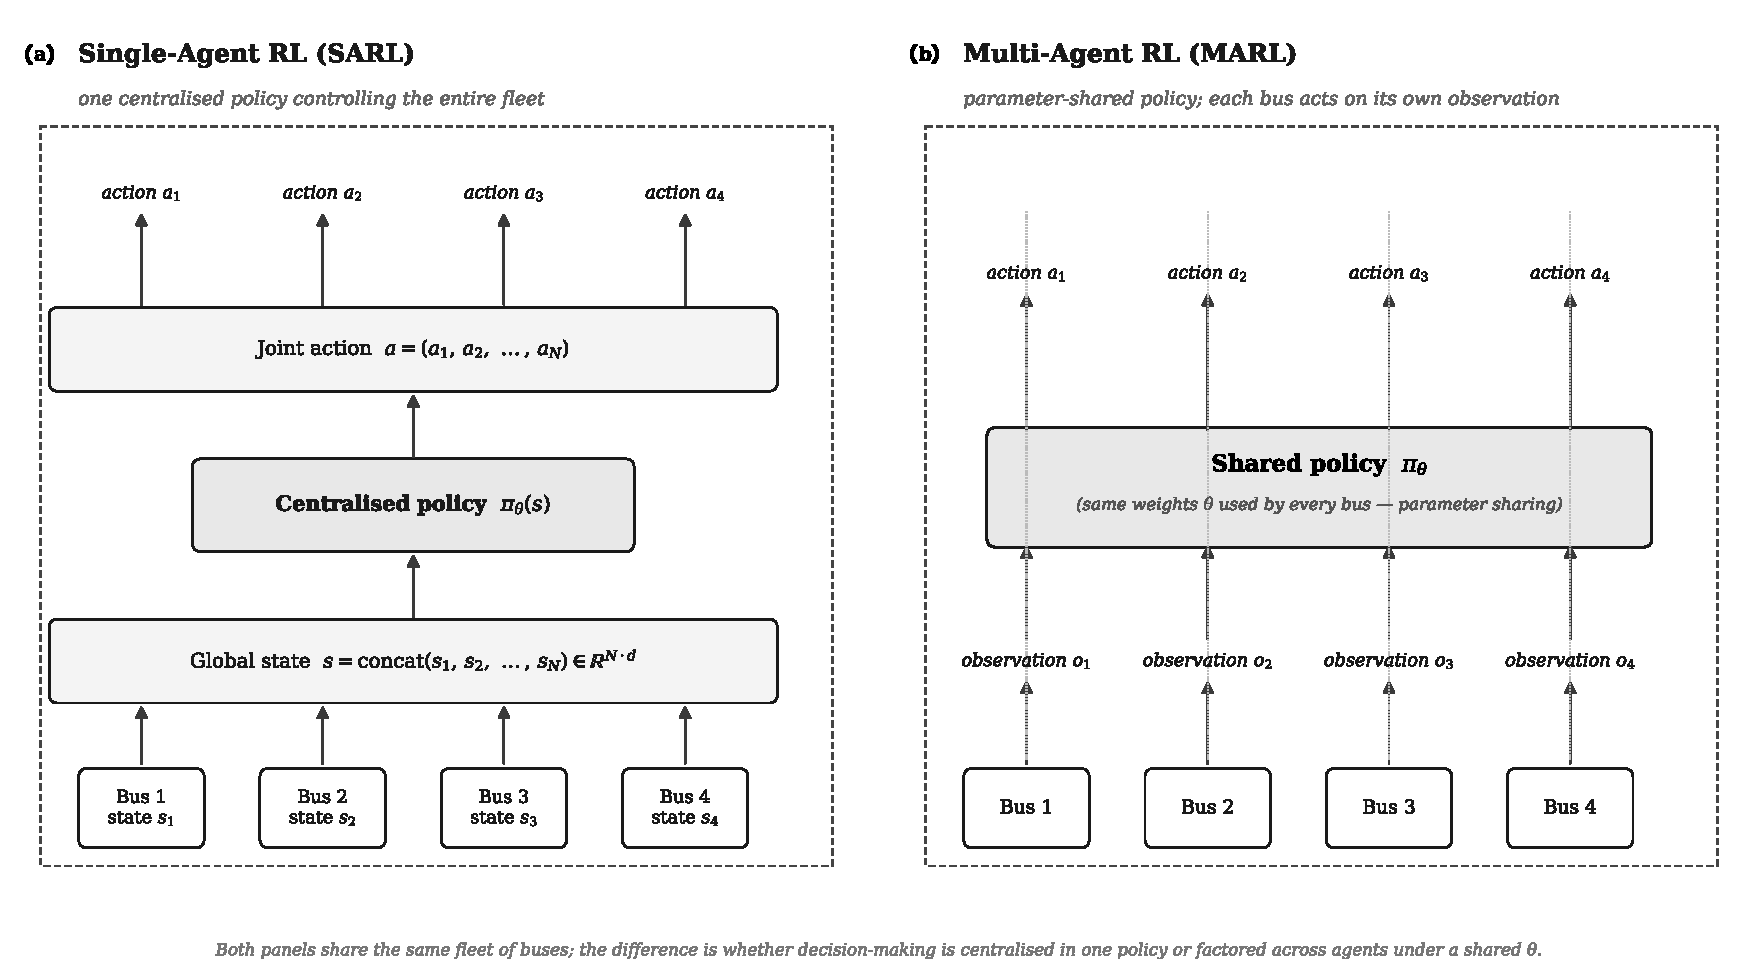
\includegraphics[clip, trim=0.1cm 0.7cm 0.1cm 0.1cm,width=\textwidth]{Figures/rrl_fig1_sarl_vs_marl (3).pdf}
    \caption[SARL vs MARL architecture]{Comparison of single-agent and
    multi-agent formulations. (a) SARL: a centralized
    policy $\pi_\theta(s)$ consumes the concatenated global state
    $s \in \mathbb{R}^{N \cdot d}$ and outputs a joint action covering every bus.
    (b) MARL with parameter sharing: a single set of weights $\theta$ is shared
    across $N$ agents, each acting on its own local observation $o_i$. Authors' illustration.}
    \label{fig:sarl-vs-marl}
\end{figure}

In both panels of Figure~\ref{fig:sarl-vs-marl}, the per-bus state (denoted $s_{i,t}$ in the formal MDP notation of Section~\ref{subsec:state-space}, and shown in the figure as the local observation $o_i$) encodes the bus's current position, forward and backward headways, onboard load, and queue length at its current stop, as defined in full in Section~\ref{subsec:state-space}. The action $a_{i,t}$ is the holding-strength and stop-skipping decision the controller emits for that bus, defined in Section~\ref{subsec:action-space}. In the SARL panel (a), a single centralized network ingests all $N$ per-bus state vectors concatenated into one global state $s \in \mathbb{R}^{N \cdot d}$ and outputs all $N$ actions simultaneously; in the MARL panel (b), the same shared network weights $\theta$ instead process each bus's local state independently, so each agent acts on only its own observation rather than the concatenated global one.

Multi-Agent Reinforcement Learning (MARL) addresses the three limitations above by decomposing decision-making across multiple agents that share the environment. Each limitation has a direct design counterpart in MARL: state-space growth is contained by giving each agent only its own \textit{local} observation rather than the global state; action-space growth is factorized by having each agent select only its own action; and the sample-inefficiency problem is mitigated by sharing one network's parameters across all agents, so that every agent's experience updates the same policy. The problem is typically formalized as a Markov Game built on an underlying Markov Decision Process, with each agent maintaining its own local observation and acting under a shared or coordinated policy \cite{Li2023Departure,Sun2024Graph,Zuo2026AGV,Huang2025Joint,Bokade2023MARL}.

This decomposition introduces a new difficulty: \textit{partial observability}. No individual bus can see the full corridor state; it knows only its own headway, load, and immediate surroundings. A fully decentralized scheme in which each agent both trains and acts on its local observation alone would be unstable, because the other agents' simultaneously evolving policies make the environment non-stationary from any one agent's viewpoint --- the same local state can transition to different outcomes depending on what the other agents happen to be learning at that moment.

To address this, most modern formulations use \textbf{Centralized Training with Decentralized Execution (CTDE)}, illustrated in Figure~\ref{fig:ctde}. During training, agents are allowed to access system-wide information and optimize a shared objective; this stabilizes learning despite the non-stationarity introduced by simultaneously adapting agents. At deployment, each bus acts only on its own local observation, which is what makes the framework practically deployable on a real fleet without requiring a centralized real-time controller \cite{Cao2022Train,Wang2024MultiAGV,Nie2025CMRM,Xu2026Hierarchical}.



\begin{figure}[htbp]
    \centering
    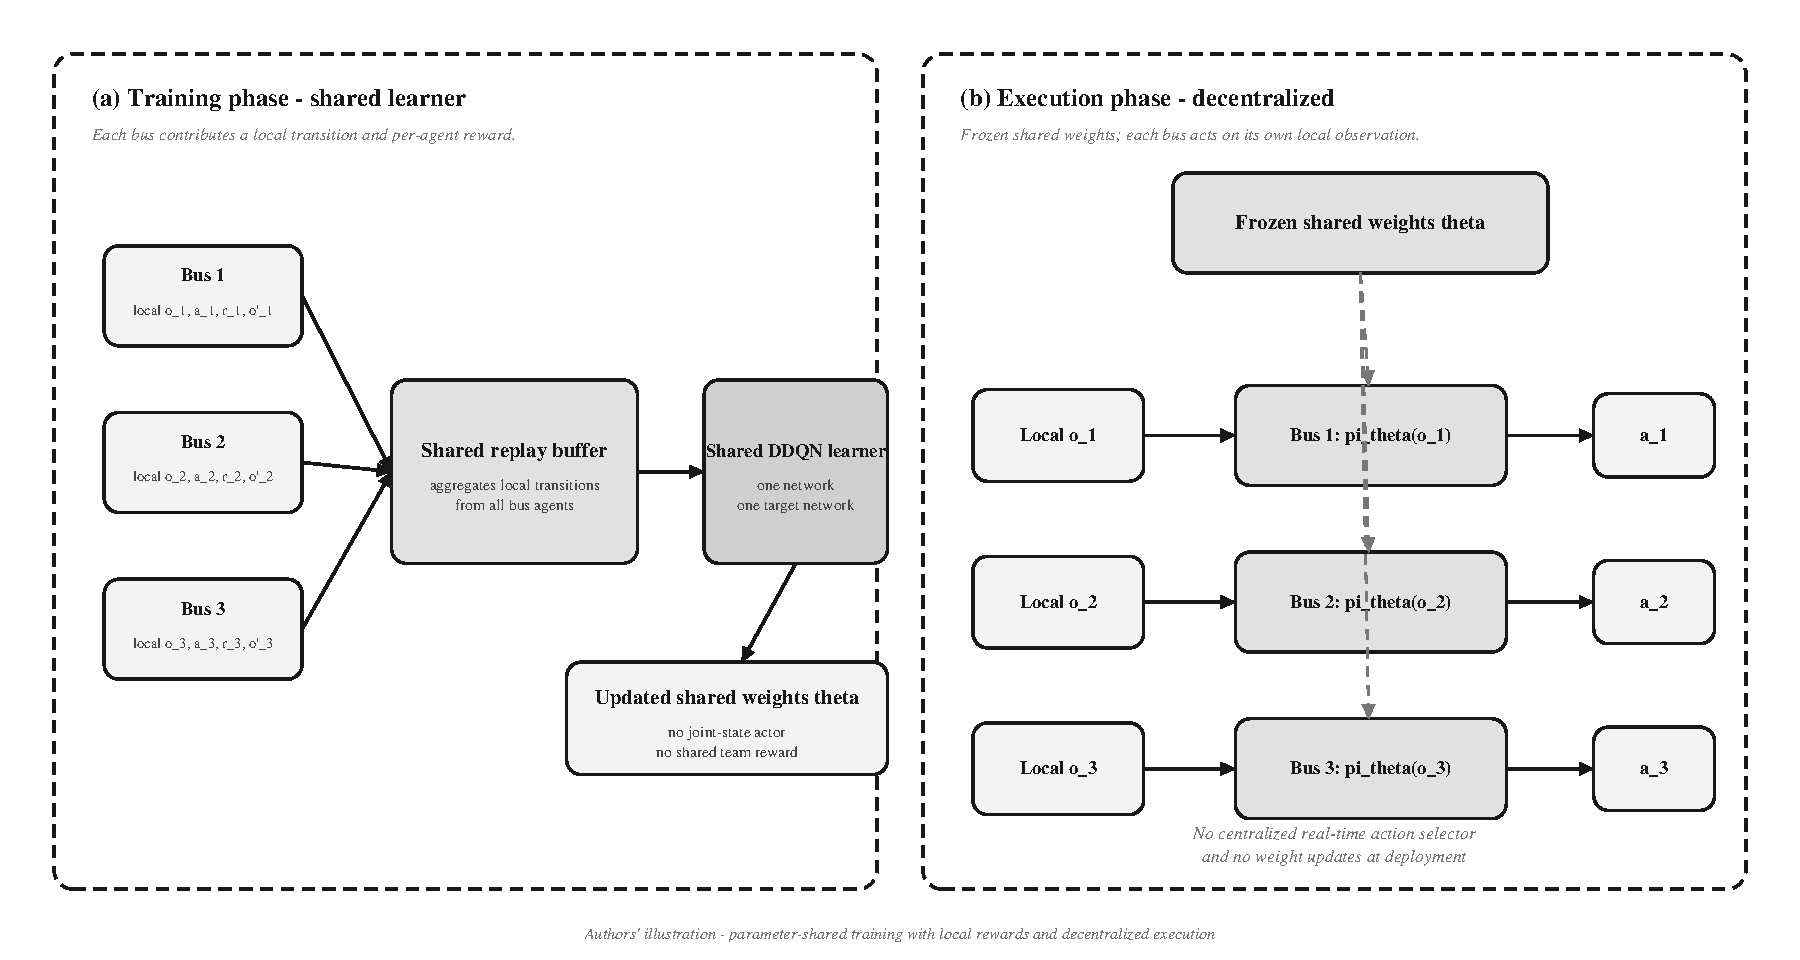
\includegraphics[width=\textwidth]{Figures/rrl_fig2_ctde (2).pdf}
    \caption[Centralized training with decentralized execution]{(a) During training, all agents share one reward
    signal and one set of policy weights $\theta$, which are updated centrally
    using joint-state information. (b) At deployment, the weights are frozen and
    each bus runs an identical copy of $\pi_\theta$ on its own local observation
    $o_i$ alone, so no centralized real-time controller is required. Authors' illustration.}
    \label{fig:ctde}
\end{figure}

In the bus-scheduling setting, a parameter-sharing CTDE architecture is fleet-size invariant: the same trained policy applies regardless of how many buses are currently in service, because every bus is an instance of the same agent class acting on its own local headway, occupancy, and queue observations. Adding or removing a bus does not invalidate the trained model. Christianos et al.~\cite{Christianos2021PS} demonstrate that parameter sharing scales effectively to large agent populations and provides empirical support for the fleet-size invariance claim.

Recent progress has combined MARL with deep learning algorithms --- Deep Q-Networks (DQN), Proximal Policy Optimization (PPO) and its multi-agent variant MAPPO, and Graph Attention Networks (GAT) --- to handle high-dimensional observation spaces and complex interactions. These have been applied across vehicle scheduling, signal control, and logistics, generally reporting improvements in routing efficiency, congestion, and throughput in simulation \cite{Li2023Departure,Cao2022Train,Wang2024MultiAGV,Sun2024Graph,Zuo2026AGV,Huang2025Joint,Bokade2023MARL}.

\subsection{MARL Applied to Bus Scheduling}
\label{subsec:marl-applied}
Within bus scheduling specifically, the MARL literature has accumulated along a recognizable trajectory: first establishing that holding control could be learned at all, then enriching the action and objective space, and most recently beginning to examine policy behavior under disturbance. This trajectory is what the present study extends.

The foundational result is due to Wang and Sun~\cite{Wang2020Holding}, who showed that a cooperative MARL framework could learn an effective bus-holding policy on a single-line corridor and outperform classical headway-equalization rules under idealized stochastic demand. Chen et al.~\cite{Chen2016MARLBus} provided an earlier proof-of-concept in the same vein on a corridor with multi-agent reinforcement learning over local headway observations. These early results established the viability of the approach but were limited to the holding action alone, restricting the policy's leverage once bunching had already developed.

Subsequent work enriched the formulation along two axes. Rodriguez et al.~\cite{Rodriguez2023Cooperative} extended the action space by combining holding with stop-skipping in a cooperative DDQN framework on a simulated transit corridor with Poisson-distributed passenger arrivals and Gaussian inter-stop travel times, reporting reductions in average passenger waiting time relative to an even-headway holding baseline. Wang and Sun~\cite{Wang2023MultiObj} extended the objective space, scaling MARL to multi-line services with a shared corridor and jointly optimizing headway regularity against operational cost under controlled simulated demand and travel-time profiles.

Recent work has increasingly examined policy behavior under disturbance. Wang and Sun's IQNC-M~\cite{Wangsun} introduced implicit quantile networks and meta-learning for risk-sensitive bus holding, evaluating performance under demand surges and traffic-speed perturbations but not under weather-induced heavy-tailed delays or discrete vehicle breakdowns. In adjacent settings, Katzilieris et al.~\cite{Katzilieris2026MARL} integrated MADDPG-based traffic signal control with dynamic bus lane access management on a simulated arterial network with deterministic signal cycles; Liu et al.~\cite{Liu2023DRLHolding} reported DRL-based holding control under stochastic travel time and demand; and Shi et al.~\cite{Shi2022DistDRL} reported a distributed DRL bus control system in a connected environment with breakdown events modeled but without weather effects.

Across this trajectory, the simulation environments share three idealizing assumptions: passenger arrivals are stationary Poisson processes, inter-stop travel times are symmetric and well-behaved (Gaussian or similar), and the fleet experiences no discrete failure events. Reported performance gains are therefore conditional on those assumptions holding at deployment. The EDSA Carousel sub-corridor studied here violates each of them. Travel times are highly non-stationary, with tail behavior driven by tropical-cyclone and heavy-rainfall events that suspend operations entirely on the most severe days \cite{DOTr2020Suspension}; passenger demand swings sharply across peak intervals, with single-day ridership peaks roughly $1.8\times$ the daily average \cite{DOTr2025Ridership}; and tight headways mean that any individual vehicle breakdown propagates through the corridor as a downstream demand-absorption problem rather than as an isolated event. A controller whose reported gains rest on the idealizing assumptions above has no validated behavior on a corridor that violates all three at once.

\begin{table}[htbp]
\centering
\caption{Disturbance coverage across MARL bus-scheduling literature.}
\label{tab:marl_performance}

\footnotesize
\renewcommand{\arraystretch}{1.3}

\begin{tabularx}{\textwidth}{
>{\RaggedRight\arraybackslash}p{2.5cm}
>{\RaggedRight\arraybackslash}p{3.0cm}
>{\RaggedRight\arraybackslash}p{2.8cm}
>{\Centering\arraybackslash}p{2.2cm}
>{\RaggedRight\arraybackslash}X
}

\toprule
\textbf{Paper} &
\textbf{Algorithm} &
\textbf{Environment} &
\textbf{Disturbances} &
\textbf{Reported gain} \\
\midrule

Wang \& Sun (2020)~\cite{Wang2020Holding} &
Cooperative MARL holding &
Single-line, idealized &
D &
Bunching reduction vs.\ headway rule \\

Chen et al.\ (2016)~\cite{Chen2016MARLBus} &
Early MARL holding &
Corridor, idealized &
D &
Proof-of-concept gains \\

Rodriguez et al.\ (2023)~\cite{Rodriguez2023Cooperative} &
Cooperative DDQN (hybrid action) &
Chicago, mesoscopic &
T &
Wait time vs.\ headway-control baseline \\

Wang \& Sun (2023)~\cite{Wang2023MultiObj} &
Multi-objective MARL &
Shared corridor, idealized &
D &
Multi-line bunching reduction \\

Wang \& Sun (2023)~\cite{Wangsun} &
IQNC-M (distributional) &
Real-world bus services &
S, T &
Stable control under extreme events \\

Katzilieris et al.\ (2026)~\cite{Katzilieris2026MARL} &
MADDPG &
Athens arterial, SUMO &
T &
Throughput improvement \\

Liu et al.\ (2023)~\cite{Liu2023DRLHolding} &
DRL holding &
Synthetic single line &
D, T &
Wait time vs.\ no-control \\

Shi et al.\ (2022)~\cite{Shi2022DistDRL} &
Distributed DRL &
Connected environment &
D, B &
Integrated control gains \\

\textbf{This study} &
\textbf{DDQN + PS (CTDE)} &
\textbf{Calibrated EDSA SUMO} &
\textbf{S, T, W, B} &
\textbf{To be evaluated} \\

\bottomrule
\addlinespace[2pt]
\multicolumn{5}{@{}p{\textwidth}@{}}{\footnotesize D~=~stochastic demand, S~=~demand surges, T~=~traffic-speed perturbation, W~=~weather-induced heavy-tail delay, B~=~discrete vehicle breakdown.} \\
\end{tabularx}
\end{table}

\clearpage
Only Shi et al.~\cite{Shi2022DistDRL} carries a B (breakdown) entry in Table~\ref{tab:marl_performance}. Cao et al.~\cite{Cao2022Train}, which also models discrete vehicle failures, is deliberately excluded from this count: their MARL application is to \textit{train} rescheduling, not bus scheduling, so it does not belong in a table scoped to MARL bus-control literature. Verbich and El-Geneidy~\cite{verbich2021} likewise model breakdowns but use heuristic, non-MARL control (Table~\ref{tab:ml_sarl_coverage}), so they are excluded for the same reason. Among MARL bus-scheduling studies specifically, Shi et al. remains the only one to model discrete breakdowns.

Table~\ref{tab:marl_performance} summarizes what each study evaluated, what disturbances it modeled, and what it reported. No prior MARL bus paper has evaluated controller performance under a framework that incorporates all four disturbance classes documented in the EDSA corridor's operational profile such as demand surges, traffic-speed variability, heavy-tailed weather-induced travel-time delays, and discrete breakdowns in a calibrated real-corridor microsimulation. Of these four, weather-induced heavy-tailed delays and discrete breakdowns are the two that no prior MARL bus-scheduling study has modeled at all; their combination with demand surges and a calibrated traffic-speed baseline is the specific disturbance profile introduced here. The algorithmic choice this study adopts to address that combined-disturbance setting, DDQN with parameter sharing under CTDE is justified in detail in Chapter~3 (Section~\ref{subsec:proposed-algorithm}), alongside the rationale for not using actor-critic or distributional alternatives. The action space the agents operate on is correspondingly small and discrete: at each control event, an agent selects a holding strength from a five-bin discretization $\alpha \in \{0.0, 0.1, 0.2, 0.3, 0.4\}$ (multiplied by a maximum holding duration to yield seconds held) combined with a binary decision to skip the next stop, giving $|A_i| = 10$ actions per event. The full action-space rationale, including why discretization is preferred over a continuous holding parameter, is given in Chapter~3 (Section~\ref{subsec:action-space}).



Under the non-ideal evaluation regime the weather generator (W) \textbf{replaces} the traffic-speed generator (T) as the source of inter-stop travel-time variability rather than acting alongside it. Both are anchored to the same per-segment empirical mean $\mu$, and the weather coefficient of variation ($\eta \ge 0.3$) already spans and exceeds the $\pm 20\%$ range produced by traffic-speed scaling (Section~3.2.6). T therefore governs travel-time stochasticity under the ideal regime and W governs it under the non-ideal regime; the two are not composed on the same segment.



\subsection{The Disturbance Gap}
\label{subsec:disturbance-gap}
The idealized assumptions in Table~\ref{tab:marl_performance} limit how confidently the reported MARL gains can be expected to transfer to real urban corridors. Real corridors violate all three assumptions: demand exhibits non-stationary surges, weather-induced travel times are skewed and heavy-tailed, and individual buses break down stochastically. Wang and Sun themselves identify this as central, noting that existing MARL bus-control studies overlook performance under perturbations and that this becomes critical when transferring models toward real-world deployment \cite{Wangsun}. Their IQNC-M framework is among the first to address demand surges and traffic-speed perturbations in bus holding control, but weather-induced heavy-tailed delays and discrete vehicle breakdowns remain outside its tested scenario set.

Two considerations explain why the gap has persisted:

\begin{enumerate}
\item \textbf{Training instability under heavy-tailed returns.} Prior MARL bus-scheduling studies have typically used Poisson arrivals and Gaussian travel-time noise because these distributions generally produce more statistically stable training behavior than heavy-tailed disturbances. In reinforcement learning literature, heavy-tailed returns and stochastic gradients are known to introduce convergence difficulties and unstable optimization behavior during policy learning \cite{Henderson2018Matters,Agarwal2021Precipice}.
\clearpage
\item \textbf{Lack of temporally aligned anomaly data.} Historical severe-weather records are rarely aligned with operational bus data at the per-segment granularity needed for direct parameter estimation, making it difficult to fit an empirically grounded heavy-tailed disturbance distribution from corridor-specific data alone, especially given the short operational observation windows typically available. \textit{This study addresses the obstacle by adopting the lognormal travel-time parameterization that Patil et al.\ \cite{Patil2025Conformal} validated against INRIX freeway data via the Kolmogorov-Smirnov test, and then sweeping the disturbance intensity across a range of validated and extrapolated CV values rather than fitting a single point estimate. This characterizes controller behavior as a function of disturbance magnitude and avoids reliance on a corridor-specific severe-weather sample whose variance cannot be reliably resolved from a short observation window.}
\end{enumerate}

\subsection{Significance of Closing the Gap}
This study contributes the first characterization of MARL bus-scheduling performance across a swept range of disturbance intensities on a calibrated real-corridor simulation, with the disturbance set covering heavy-tailed weather-induced travel-time delays and discrete bus breakdowns that no prior MARL bus-scheduling study has modeled. Understanding policy performance under disturbance matters for two reasons. First, deploying MARL bus-scheduling models on the basis of ideal-simulator benchmarks alone leaves their real-world failure modes unknown until deployment, which is an unacceptable risk profile for a system that carries hundreds of thousands of daily passengers. Second, the relevant performance question for transit operators is not only average-case waiting time under quiet conditions but how a control policy degrades as a disruption intensifies, a characterization that prior MARL bus-scheduling work does not report. Establishing a reproducible stress-testing protocol pairing a calibrated corridor simulation with configurable demand, weather, and breakdown generators therefore contributes both an empirical characterization of performance under disturbance and a reusable evaluation framework for subsequent MARL work in this domain \cite{Li2023Departure,Wang2024MultiAGV,Che2024Recharging,Huang2025Joint,Bokade2023MARL}.